\chapter{Development}\label{ch:development}
\lstset{style=inline}

\section{Project Inception}
The initial concept for the project revolved around the use of a collection of SD-Cards, containing operating systems tailored for specific use cases.
The user would be to able insert the wanted SD-Card into the RPI, which then would execute a script on startup to configure the operating system for a specific scenario.

With the usability of this system appearing quite cumbersome, it was instead opted to develop a user interface (UI), which would execute the wanted shell scripts during runtime.
To implement the UI, it was decided on the use of a simple terminal-based interface, which would be printed directly into the shell. 
This approach would facilitate straightforward navigation through the use of a dial and push-button combination, providing an intuitive means for users to interact with the system. 
The program should be written in C or C++ due to my familiarity with both languages.

From this concept the following 3D model was created to visualize the project idea:

\begin{figure}[h]
    \centering
    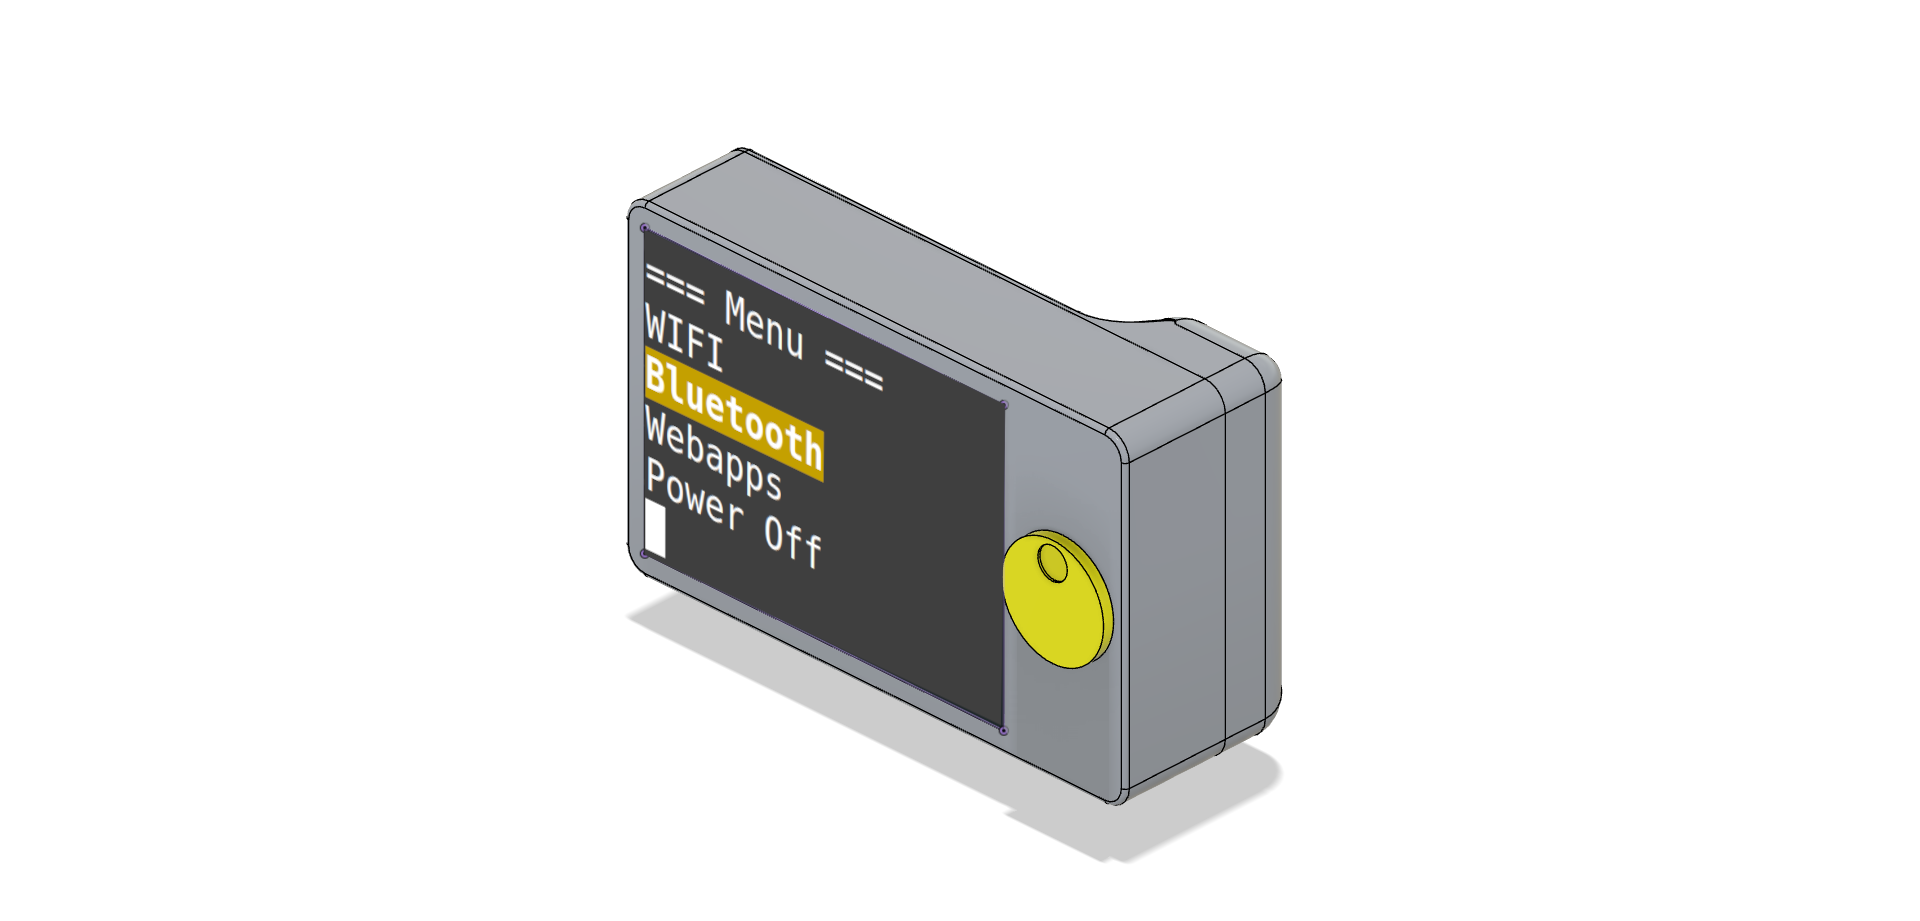
\includegraphics[width=0.7\textwidth]{figures/Abbildungen/Concept.png}
    \caption{Concept Model}
    \label{fig:concept}
\end{figure}

\section{User Interface}\label{sec:ui}
To display the UI, the menus need to be printed into the terminal, for which a simple loop, that periodically clears the screen and prints the options of a menu, was decided on.
Subsequently, a fitting software architecture needed to be designed, which can model the variety of menus and their respective options with individual actions.
The menus need to display options, which require the capability of executing various actions, including the transition to other menus and the execution of shell scripts and programs.
Since the command design pattern at this point was unknown to me, the modeling of the menus with a uniform class turned out quite challenging.
Therefore, it was decided to model the menus as classes, containing objects of the MenuOption class, and utilize the std::function for action execution.

In order for the device to be usable with the built in screen and selector dial, the RPI needs to be configured to run and display the UI program on startup.
Execution of the program on startup is implemented with the help of a systemd service.
For the setup, an according configuration file needs to be added to \textit{/etc/systemd/system}, which is activated by running the \lstinline[]|systemctl enable [service].service| command.

Instead of a BIOS\footnote{Binary Input Output System: boots before the OS}, the RPI employs a configuration file (\textit{/boot/firmware/config.txt}), which is read on startup to initialize the hardware and operating system.
To this file the following lines were added:

\begin{lstlisting}[numbers=none, frame=none]
    dtoverlay=waveshare35a
    framebuffer_width=200
    framebuffer_height=120 
\end{lstlisting}

Line one sets up a hardware overlay to initialize the display, lines two and three set the resolution of the display.
With the resolution set to the factory specification of 800x480, the UI is displayed quite small, thus poorly suited for the use case.
Since the OS runs in terminal without a graphic server, there is no simple option for scaling the UI.
The scale problem was fixed with a workaround, which involves the resolution inside the \textit{config.txt} to be set to 200x120, therefore forcing the UI to scale.
The increased scale leads to the menus being clearly readable and comfortable to use, but limits the readability of console output.

Initially it was planned to use the display in vertical orientation, however, attempts to rotate the terminal by configuration inside \textit{config.txt} or the kernel command line (\textit{/boot/firmware/cmdline.txt}) were unsuccessful.

\section{Network Management}\label{sec:network_management}
For network management, it was decided on use of the Network Manager Command Line Interface (nmcli) tool, which is easy to use and offers a sizable set of configuration options and utilities.
At the start of the development of the shell scripts for Wi-Fi activation, it was unclear, how to configure a connection in line with the specification of the different Wi-Fi standards.
After research on the different security mechanisms and the nmcli documentation was conducted, the solution appeared to be the manual configuration of the encryption algorithm, key management, and information element for each connection.

The script developed for changing Wi-Fi passwords was designed to utilize a password list, from which a random password would be extracted for the connection. 
However, large password lists, such as the RockYou list included in Kali Linux\footnote{see \cref{sec:testing_methods}}, proved impractical due to their considerable size, complicating handling.
A password list containing 100,000 entries was selected as the data source. 
Given the varying requirements for passwords across different Wi-Fi standards, as detailed in \cref{ch:documentation}, the list contained a number of unsuitable entries.
It was subsequently filtered using a simple script (see listing \ref{lst:passwdExtract}) to generate password lists that conformed to the specific requirements of each standard.

\lstinputlisting[style=block, language=bash, caption={script for password extraction}, label={lst:passwdExtract}]{listings/Raspi-CyberSec-Lab-Project/Passwords/extract.sh}

For the Wi-Fi status function, the \lstinline[breaklines=true]|nmcli dev wifi show-password ifname [device name]| command is employed to display the type of network, its SSID and password.
\\Unfortunately this command is not functional for WEP networks, therefore a script was created, which extracts the SSID and password from \textit{/etc/NetworkManager/system-connections}, formatted to output alike the nmcli utility.

In the implementation of the Wi-Fi monitor function, the objective was to create a logger that would enable users to trace the events of an attack, such as the dis-/connection of devices and any changes to the network.
The command \lstinline[]|iw event -T| provides timestamps and MAC addresses for devices connecting to or disconnecting from the network. 
Additionally, \lstinline[]|nmcli monitor| reports any modifications made to the network status but does not include timestamps in its output. 
Attempts to add timestamps by using \lstinline[]|awk| or \lstinline[]|ts| were unsuccessful, as nmcli monitor must be executed in the background to allow the UI to remain operational. 
Furthermore, a challenge that remains unresolved is the integration of the outputs from both programs into a single log file.

As described in \cref{sec:results}, some critical configuration errors were discovered during the testing process.
In the pursuit of fixing the configuration errors, the WPA network was accidentally configured to use enterprise authentication in the form on 801.2X.
Switching the configuration back to WPA-PSK, the Wi-Fi connection continued trying to reach the server for enterprise authentication during activation, timing out with the error message:

\begin{lstlisting}[style=block, numbers=none]
Error: Connection activation failed: 802.1X supplicant took too long to authenticate 
Hint: use 'journalctl -xe NM_CONNECTION=7fb3feca-d2b4-424a-85ee-e0aa40f1c90a + NM_DEVICE=wlan1' to get more details.
\end{lstlisting}

After allocation of significant time and the discovery of more unexpected behavior with \lstinline[]|nmcli|, it was decided to create a new OS setup on another SD card.

For the correct setup of the WEP network, the following lines were added or modified:
\lstinputlisting[style=block,language=bash,linerange={13-14, 16-16},numbers=none,tabsize=1,label={lst:fix_WEP}]{listings/Raspi-CyberSec-Lab-Project/Skripte/wifiActivate.sh}

With the renewed OS setup, the connection timeout for the WPA supplicant seemed to be resolved, and WPA and WPA2 connections were correctly established.

However, on the second pentest of the WPA network, the supplicant error appeared once again, even though enterprise authentication was never activated, which leads to the assumption that this error is being caused by a software bug.

The final solution found involves the WPA supplicant being disabled by executing
\\\lstinline[]|systemctl disable wpa_supplicant|.
This allows the activation of the WPA network, although the error still appears occasionally.
A reliable fix for the problem could not be determined at this point.

\section{Rotary Encoder}
To use the encoder dial as a scroll wheel, its signals need to be processed and translated to instructions for the main program to execute.
After the encoder was soldered to a simple circuit of pull-up resistors and connected to the GPIO pins of the RPI, the encoder program was developed for processing the encoder's outputs.

Off the shelf rotary encoders incorporate clicks into their rotation, similar to the scrolling wheel of a computer mouse, and output two digital signals.
These signals are called DT and CLK, which, when turned, oscillate with 90 degrees of phase shift, resulting in a Gray code with two bits (see \cref{fig:encoder_processing}).
Through saving the previous state and comparing it to the new state, once the encoder was turned, the direction of rotation can be determined.
According to various online source, this kind of encoders switch one state on each click, like the dotted arrow in \cref{fig:encoder_processing} depicts.

\begin{figure}[h]
   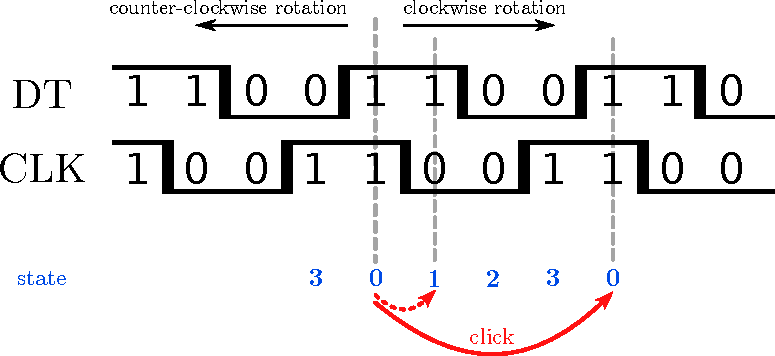
\includegraphics[width=0.7\textwidth]{figures/Abbildungen/encoder.pdf} 
   \centering
   \caption{Encoder Processing}
   \label{fig:encoder_processing}
\end{figure}

During development of the encoder program, the output showed unexpected behavior, which was discovered to originate from the encoder switching through states 0 to 3 between clicks, as depicted by the red arrow in \cref{fig:encoder_processing}.
The discovery of this behavior helped to simplify the processing since this pattern allows a single query of the signal states to determine the direction of rotation.
As seen in listing \ref{lst:ISR_rotation}, the processing was then applied in a single ISR, comparing the DT and CLK signals.

\section{ESP32}
To establish communication between the RPI and the ESP32, some of the GPIO pins needed to be initialized for UART, which was achieved by adding a hardware overlay to the \textit{config.txt} file.
The code of the ESP32 in large part consists of code examples provided by the ESP-IDF GitHub (\cite{espidf}).
From these examples the code was compiled from snippets the Wi-Fi station example, MQTT web socket example and UART events example.
These snippets were modified to work in conjunction with the scripts present on the RPI.

When closing a network and reopening another, instructing the ESP32 to switch to the new network, led it to regularly crash with the error \lstinline[]|itwt_stop_process|.
After investigation, the error seemed to originate from a Wi-Fi power-saving mechanism present in Wi-Fi 6, called Target Wake Time (TWT).
Various attempts at solving the error by disabling the power saving were attempted but resulted unsuccessful.

The solution, finally implemented, involved the code being restructured to reset the MCU on a UART command, preceding the establishment of a network connection.

